\section{Ejercicio 8}

Para este ejercicio se pedía realizar tareas de prueba para comparar los schedulers \emph{Round Robin}, \emph{FCFS}, \emph{SJF} y \emph{RSJF}.

Luego, realizar comparaciones según latencia, waiting time y turnaround, realizar gráficos y tablas para exponer los resultados y dar una conclusión.

Como los schedulers \emph{SJF} y \emph{RSJF} sólo toman tareas del tipo TaskCPU, los lotes generados para los experimentos son con este tipo de tareas.

También, en los experimentos el costo de cambiar de contexto es de dos y el costo de cambiar un proceso de núcleo es de uno.

\subsection{Primera Prueba}

Para esta prueba utilizamos el lote de tareas \textbf{ej8lote1}, utilizando solamente las del tipo TaskCPU dado que es la única tarea que se puede correr en los scheluders de tipo \emph{SJF} y \emph{RSJF}, así se puede realizar una comparación veraz entre todos. Estas son lanzadas en al mismo tiempo a los schedulers al comienzo de la ejecución. Los tiempos tomados para ellas son 5, 7, 3, 11 y 2.

La cantidad de cores utilizados en este caso es de uno. Y, en el caso de \emph{Round Robin} y \emph{RSJF}, el quantum dado es 3.

Lo que intentamos ver en esta prueba es, dado este lote de tareas, el comportamiento, velocidad en ejecutar y terminar estas con los schedulers implementados.

Los gráficos obtenidos son:

\begin{figure}[!h]
	\begin{center}
		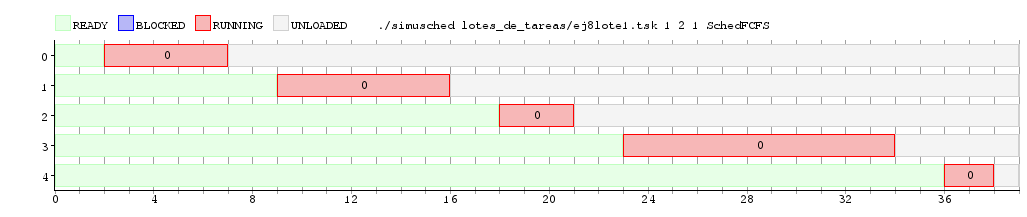
\includegraphics[width=500px]{imagenes/ej8_prueba1_fcfs.png}
		\caption{Ejecución del lote \emph{ej8lote1} con scheduler FCFS.}
		\label{fig:grafico_ej8_prueba1_fcfs}
	\end{center}
\end{figure}

\begin{figure}[!h]
	\begin{center}
		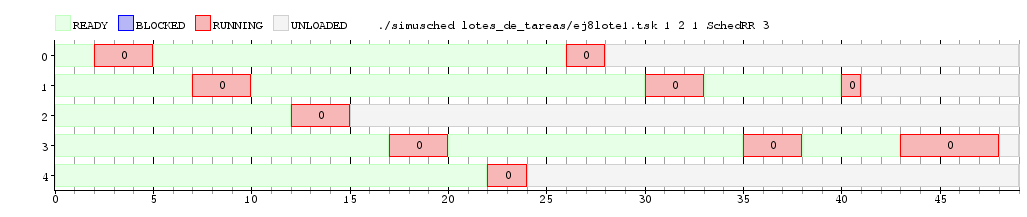
\includegraphics[width=500px]{imagenes/ej8_prueba1_rr.png}
		\caption{Ejecución del lote \emph{ej8lote1} con scheduler Round Robin.}
		\label{fig:grafico_ej8_prueba1_rr}
	\end{center}
\end{figure}

\begin{figure}[!h]
	\begin{center}
		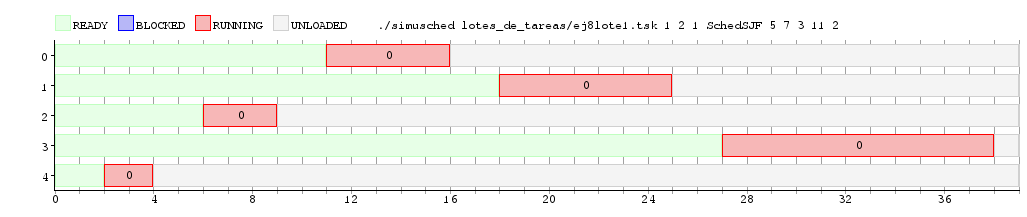
\includegraphics[width=500px]{imagenes/ej8_prueba1_sjf.png}
		\caption{Ejecución del lote \emph{ej8lote1} con scheduler SJF.}
		\label{fig:grafico_ej8_prueba1_sjf}
	\end{center}
\end{figure}

\begin{figure}[!h]
	\begin{center}
		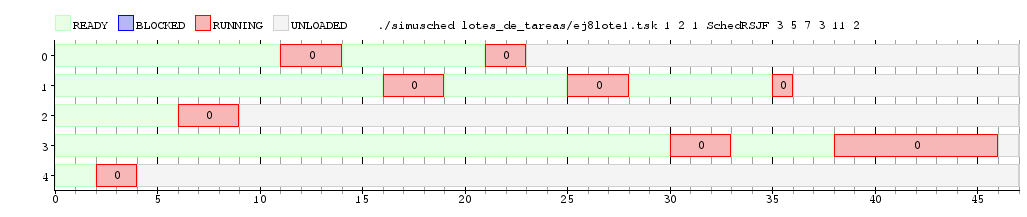
\includegraphics[width=500px]{imagenes/ej8_prueba1_rsjf.png}
		\caption{Ejecución del lote \emph{ej8lote1} con scheduler RSJF.}
		\label{fig:grafico_ej8_prueba1_rsjf}
	\end{center}
\end{figure}

\newpage

%LATENCIA PROMEDIO
\begin{center}
	\begin{tabular}{|c|c|c|c|}
		\hline
		\multicolumn{4}{|c|}{\large{\textbf{Latencia Promedio}}} \\
		\hline
		\textbf{FCFS} & \textbf{Round Robin} & \textbf{SJF} & \textbf{RSJF} \\
		\hline
		17,6 & 12 & 12,8 & 13 \\
		\hline
	\end{tabular}
\end{center}

%WAITING TIME PROMEDIO
\begin{center}
	\begin{tabular}{|c|c|c|c|}
		\hline
		\multicolumn{4}{|c|}{\large{\textbf{Waiting Time Promedio}}} \\
		\hline
		\textbf{FCFS} & \textbf{Round Robin} & \textbf{SJF} & \textbf{RSJF} \\
		\hline
		17,6 & 25,6 & 12,8 & 18 \\
		\hline
	\end{tabular}
\end{center}

%TIEMPO TOTAL DE EJECUCION PROMEDIO
\begin{center}
	\begin{tabular}{|c|c|c|c|}
		\hline
		\multicolumn{4}{|c|}{\large{\textbf{Tiempo Total De Ejecución Promedio}}} \\
		\hline
		\textbf{FCFS} & \textbf{Round Robin} & \textbf{SJF} & \textbf{RSJF} \\
		\hline
		23,2 & 31,2 & 18,4 & 23,6 \\
		\hline
	\end{tabular}
\end{center}

Cómo podemos observar por los cálculos, la latencia del scheduler \emph{FCFS} para este lote de tareas fue el que tuvo el promedio mayor. Esto se debe a que este toma un proceso y lo corre hasta terminar y eso hace esperar a los demás procesos en la cola. En cuanto a los demás schedulers, \emph{Round Robin} fue la menor, tuvo la menor latencia, esto se debe a que, como su quantum era 3, la espera para los demás procesos era mas corta. \emph{SJF} y \emph{RSJF} se comportaron de una forma similar y cercana, tanto entre si como con \emph{Round Robin}.

Sobre el waiting time, \emph{Round Robin} fue el scheduler con el promedio mas alto, esto se debe a que, al desalojar los procesos en un quantum fijo hace que genere mas tiempo de espera hasta que terminan. El scheduler con menor waiting time promedio fue \emph{SJF}, al elegir siempre el proceso con el menor tiempo y ejecutarlo hasta terminar genera que tenga menos desalojos. Esto no sucede con \emph{RSJF}, aunque elija el proceso con el menor tiempo para terminar, depende mucho del quantum que posee que, mientras más chico es, más desalojos va a tener (siempre tomando en cuenta que los procesos tienen más tiempo de ejecución que quantum) y esto hace que aumente.

Sobre el tiempo total de ejecución, son muy similares a los del waiting time, y se debe a los motivos descriptos.

Luego de realizar estas comparaciones, decidímos realizar la misma prueba pero esta vez con dos cores en cada scheduler para ver cómo mejora su performance. En los schedulers \emph{Round Robin} y \emph{RSJF} el quantum de ambos cores es de tres (lo mantuvimos igual).

\begin{figure}[!h]
	\begin{center}
		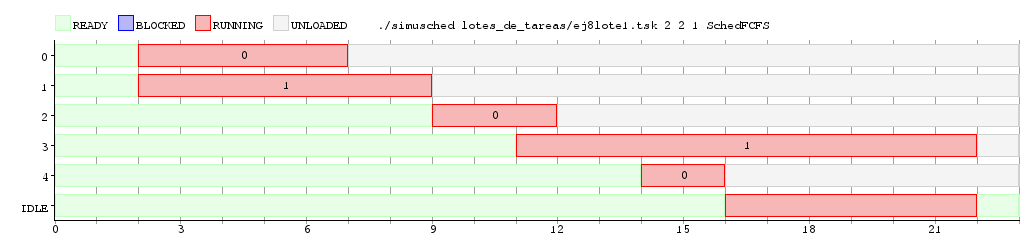
\includegraphics[width=500px]{imagenes/ej8_prueba1_fcfs2.png}
		\caption{Ejecución del lote \emph{ej8lote1} con scheduler FCFS con 2 cores.}
		\label{fig:grafico_ej8_prueba1_fcfs2}
	\end{center}
\end{figure}

\newpage

\begin{figure}[!h]
	\begin{center}
		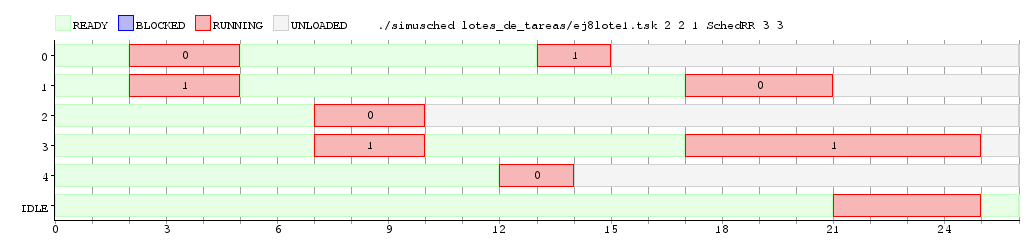
\includegraphics[width=500px]{imagenes/ej8_prueba1_rr2.png}
		\caption{Ejecución del lote \emph{ej8lote1} con scheduler Round Robin con dos cores.}
		\label{fig:grafico_ej8_prueba1_rr2}
	\end{center}
\end{figure}

\begin{figure}[!h]
	\begin{center}
		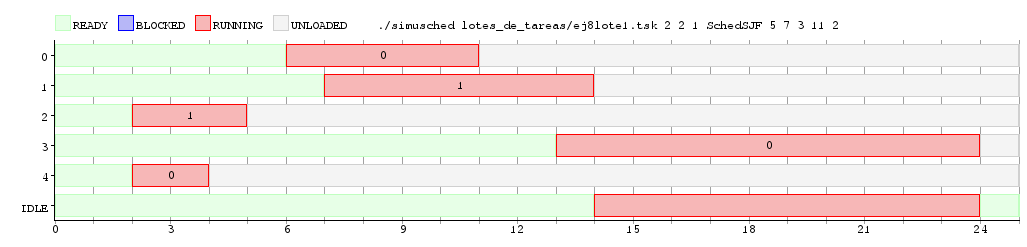
\includegraphics[width=500px]{imagenes/ej8_prueba1_sjf2.png}
		\caption{Ejecución del lote \emph{ej8lote1} con scheduler SJF con dos cores.}
		\label{fig:grafico_ej8_prueba1_sjf2}
	\end{center}
\end{figure}

\begin{figure}[!h]
	\begin{center}
		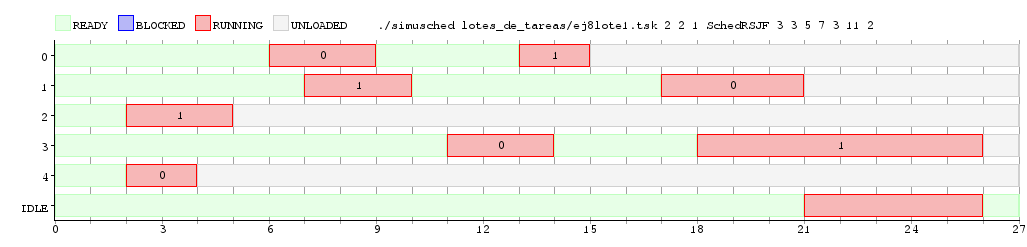
\includegraphics[width=500px]{imagenes/ej8_prueba1_rsjf2.png}
		\caption{Ejecución del lote \emph{ej8lote1} con scheduler RSJF con dos cores.}
		\label{fig:grafico_ej8_prueba1_rsjf2}
	\end{center}
\end{figure}

%LATENCIA PROMEDIO
\begin{center}
	\begin{tabular}{|c|c|c|c|}
		\hline
		\multicolumn{4}{|c|}{\large{\textbf{Latencia Promedio}}} \\
		\hline
		\textbf{FCFS} & \textbf{Round Robin} & \textbf{SJF} & \textbf{RSJF} \\
		\hline
		7,6 & 6 & 6 & 5,6 \\
		\hline
	\end{tabular}
\end{center}

%WAITING TIME PROMEDIO
\begin{center}
	\begin{tabular}{|c|c|c|c|}
		\hline
		\multicolumn{4}{|c|}{\large{\textbf{Waiting Time Promedio}}} \\
		\hline
		\textbf{FCFS} & \textbf{Round Robin} & \textbf{SJF} & \textbf{RSJF} \\
		\hline
		7,6 & 11,4 & 6 & 8,6 \\
		\hline
	\end{tabular}
\end{center}

%TIEMPO TOTAL DE EJECUCION PROMEDIO
\begin{center}
	\begin{tabular}{|c|c|c|c|}
		\hline
		\multicolumn{4}{|c|}{\large{\textbf{Tiempo Total De Ejecución Promedio}}} \\
		\hline
		\textbf{FCFS} & \textbf{Round Robin} & \textbf{SJF} & \textbf{RSJF} \\
		\hline
		13,2 & 17 & 11,6 & 14,2 \\
		\hline
	\end{tabular}
\end{center}

Al aumentar un core, podemos comprobar que la performance de cada scheduler mejoró en un 50\% aproximadamente, con algunos valores que superaron el valor. En promedio, las diferencias entre ellos se mantuvieron igual que con un core pero la mejora de performance en tiempos es notoria.

\subsection{Segunda Prueba}

Para esta prueba utilizamos el lote de tareas \textbf{ej8lote2}, utilizando las mismas tareas sólo que estas son lanzadas con una diferencia de dos ticks desde el comienzo de la ejecución. Esto se realizo para poder comparar la performance de los distintos schedulers tanto con tareas que ingresan simultaneamente como tareas que llegan en distinto momento como en este caso.

En esta prueba, como la anterior, comenzamos utilizando un core por scheduler y, para los schedulers \emph{Round Robin} y \emph{RSJF}, el quantum dado es 3.

La cantidad de cores utilizados en este caso es de uno. Y, en el caso de \emph{Round Robin} y \emph{RSJF}, el quantum dado es 3.

En este caso, intentamos ver el comportamiento de los schedulers en donde las tareas van apareciendo con una frecuencia constante.

Los gráficos obtenidos son:

\begin{figure}[!h]
	\begin{center}
		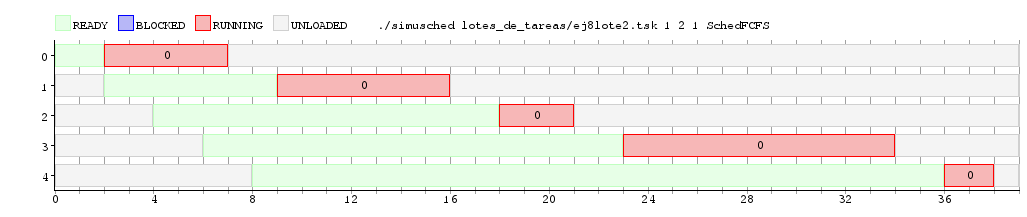
\includegraphics[width=500px]{imagenes/ej8_prueba2_fcfs.png}
		\caption{Ejecución del lote \emph{ej8lote2} con scheduler FCFS.}
		\label{fig:grafico_ej8_prueba2_fcfs}
	\end{center}
\end{figure}

\begin{figure}[!h]
	\begin{center}
		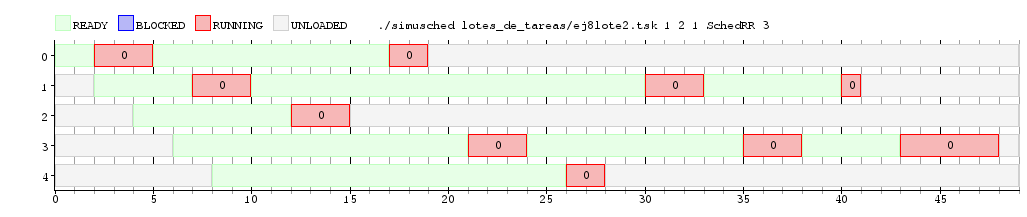
\includegraphics[width=500px]{imagenes/ej8_prueba2_rr.png}
		\caption{Ejecución del lote \emph{ej8lote2} con scheduler Round Robin.}
		\label{fig:grafico_ej8_prueba2_rr}
	\end{center}
\end{figure}

\begin{figure}[!h]
	\begin{center}
		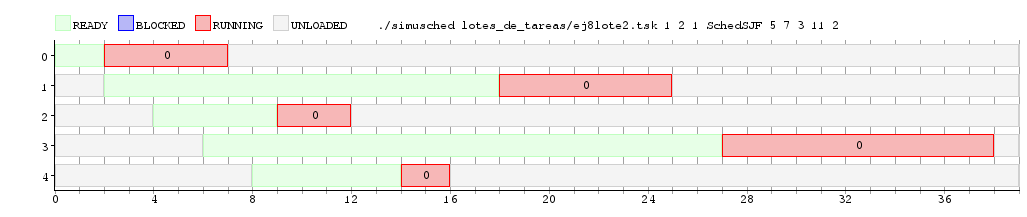
\includegraphics[width=500px]{imagenes/ej8_prueba2_sjf.png}
		\caption{Ejecución del lote \emph{ej8lote2} con scheduler SJF.}
		\label{fig:grafico_ej8_prueba2_sjf}
	\end{center}
\end{figure}

\newpage

\begin{figure}[!h]
	\begin{center}
		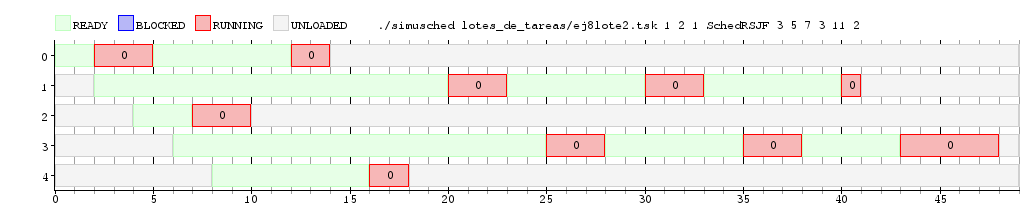
\includegraphics[width=500px]{imagenes/ej8_prueba2_rsjf.png}
		\caption{Ejecución del lote \emph{ej8lote2} con scheduler RSJF.}
		\label{fig:grafico_ej8_prueba2_rsjf}
	\end{center}
\end{figure}

%LATENCIA PROMEDIO
\begin{center}
	\begin{tabular}{|c|c|c|c|}
		\hline
		\multicolumn{4}{|c|}{\large{\textbf{Latencia Promedio}}} \\
		\hline
		\textbf{FCFS} & \textbf{Round Robin} & \textbf{SJF} & \textbf{RSJF} \\
		\hline
		16,6 & 9,6 & 10 & 10,2 \\
		\hline
	\end{tabular}
\end{center}

%WAITING TIME PROMEDIO
\begin{center}
	\begin{tabular}{|c|c|c|c|}
		\hline
		\multicolumn{4}{|c|}{\large{\textbf{Waiting Time Promedio}}} \\
		\hline
		\textbf{FCFS} & \textbf{Round Robin} & \textbf{SJF} & \textbf{RSJF} \\
		\hline
		16,6 & 20,6 & 10 & 16,6 \\
		\hline
	\end{tabular}
\end{center}

%TIEMPO TOTAL DE EJECUCION PROMEDIO
\begin{center}
	\begin{tabular}{|c|c|c|c|}
		\hline
		\multicolumn{4}{|c|}{\large{\textbf{Tiempo Total De Ejecución Promedio}}} \\
		\hline
		\textbf{FCFS} & \textbf{Round Robin} & \textbf{SJF} & \textbf{RSJF} \\
		\hline
		19,2 & 26,6 & 15,6 & 22,2 \\
		\hline
	\end{tabular}
\end{center}

Los datos obtenidos sobre este lote de tareas reflejan una leve mejora con respecto a la primera prueba donde las tareas son agregadas a los schedulers en el mismo tiempo.

Sobre la latencia, \emph{Round Robin} sigue teniendo una mejor performance, seguido de cerca por \emph{SJF} y \emph{RSJF} y, \emph{FCFS} se mantuvo con la peor latencia. \emph{FCFS} podría mejorarla si procesos nuevos aparezcan una vez que termino otro, pero es un caso muy particular.

Sobre waiting time, \emph{SJF} obtuvo la mejor performance, esto se debe a que siempre corre los procesos que terminan más rápido hasta terminarlos y esto genera que el tiempo de espera sea mucho menor. \emph{Round Robin} tuvo la peor performance, esto se debe a la cantidad de procesos que posee y el quantum dado a cada uno, si se aumenta un poco el quantum podría mejorar su performance sobre el waiting time.

Sobre el tiempo total de ejecución, los valores entre sí son muy parecidos a los del waiting time, donde hicimos algunos comentarios al respecto.

Cómo en la prueba anterior, decidimos realizar esta misma prueba pero agregando un core más a cada implementación para ver cómo mejoran las performances. En los schedulers \emph{Round Robin} y \emph{RSJF} el quantum de ambos cores es de tres (lo mantuvimos igual).

\begin{figure}[!h]
	\begin{center}
		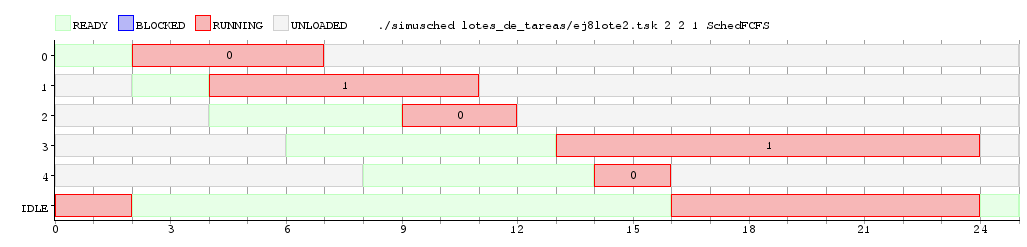
\includegraphics[width=500px]{imagenes/ej8_prueba2_fcfs2.png}
		\caption{Ejecución del lote \emph{ej8lote2} con scheduler FCFS con 2 cores.}
		\label{fig:grafico_ej8_prueba2_fcfs2}
	\end{center}
\end{figure}

\begin{figure}[!h]
	\begin{center}
		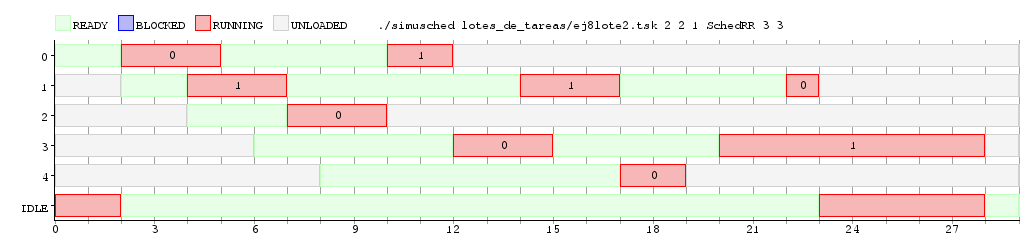
\includegraphics[width=500px]{imagenes/ej8_prueba2_rr2.png}
		\caption{Ejecución del lote \emph{ej8lote2} con scheduler Round Robin con dos cores.}
		\label{fig:grafico_ej8_prueba2_rr2}
	\end{center}
\end{figure}

\newpage

\begin{figure}[!h]
	\begin{center}
		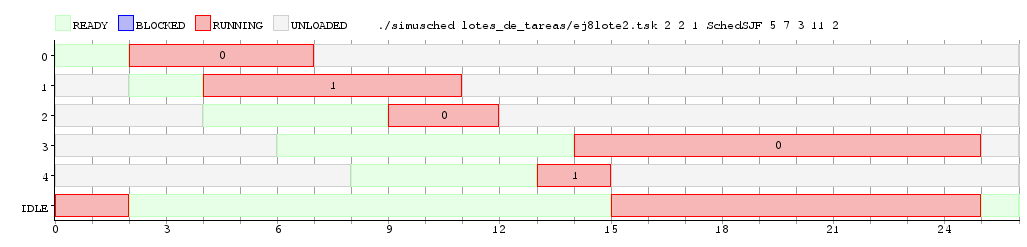
\includegraphics[width=500px]{imagenes/ej8_prueba2_sjf2.png}
		\caption{Ejecución del lote \emph{ej8lote2} con scheduler SJF con dos cores.}
		\label{fig:grafico_ej8_prueba2_sjf2}
	\end{center}
\end{figure}

\begin{figure}[!h]
	\begin{center}
		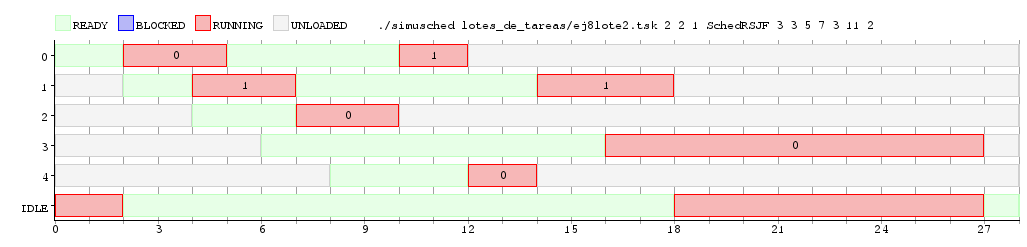
\includegraphics[width=500px]{imagenes/ej8_prueba2_rsjf2.png}
		\caption{Ejecución del lote \emph{ej8lote2} con scheduler RSJF con dos cores.}
		\label{fig:grafico_ej8_prueba2_rsjf2}
	\end{center}
\end{figure}

%LATENCIA PROMEDIO
\begin{center}
	\begin{tabular}{|c|c|c|c|}
		\hline
		\multicolumn{4}{|c|}{\large{\textbf{Latencia Promedio}}} \\
		\hline
		\textbf{FCFS} & \textbf{Round Robin} & \textbf{SJF} & \textbf{RSJF} \\
		\hline
		4,4 & 4,4 & 4,4 & 4,2 \\
		\hline
	\end{tabular}
\end{center}

%WAITING TIME PROMEDIO
\begin{center}
	\begin{tabular}{|c|c|c|c|}
		\hline
		\multicolumn{4}{|c|}{\large{\textbf{Waiting Time Promedio}}} \\
		\hline
		\textbf{FCFS} & \textbf{Round Robin} & \textbf{SJF} & \textbf{RSJF} \\
		\hline
		4,4 & 8,8 & 4,4 & 6,6 \\
		\hline
	\end{tabular}
\end{center}

%TIEMPO TOTAL DE EJECUCION PROMEDIO
\begin{center}
	\begin{tabular}{|c|c|c|c|}
		\hline
		\multicolumn{4}{|c|}{\large{\textbf{Tiempo Total De Ejecución Promedio}}} \\
		\hline
		\textbf{FCFS} & \textbf{Round Robin} & \textbf{SJF} & \textbf{RSJF} \\
		\hline
		10 & 14,4 & 10 & 12,2 \\
		\hline
	\end{tabular}
\end{center}

En esta prueba con dos cores se pudo notar que la performance mejoró también en un 50\% promedio que cuando se probó con un solo core, logrando una mejora grande sobre el scheduler \emph{FCFS}.

La latencia entre los schedulers fue similar entre los cuatro schedulers, con una leve mejora en \emph{RSJF}. Cómo no hay muchos procesos esperando cuando empiezan a correr, esto hizo que el scheduler \emph{FCFS}, el peor sobre latencia en las pruebas anteriores, mejorara mucho más que un 50\% que los demás que se mantuvieron más estables.

Sobre waiting time, \emph{Round Robin} mantuvo la peor performance pero \emph{FCFS} pudo igualar a la mejor performance que la tenía \emph{SJF} y esto se debe a lo comentado, que se vayan encolando procesos a medida que van corriendo otros genera menor tiempo de espera.

En el tiempo total de ejecución promedio también el scheduler \emph{FCFS} obtuvo una mejora de performance notoria llevándolo a obtener la mejor performance junto con \emph{SJF}. \emph{Round Robin} mantuvo la peor performance de esta comparación.

En comparación con la primer prueba podemos notar que en esta se genero una disminución en todos las métricas calculadas, sin embargo se pudo ver que los distintos schedulers se beneficiaron del cambio de distinta manera en cada métrica. En particular podemos ver que el FCFS tan solo disminuyo un 5,69\% su latencia, mientras que los demás tuvieron un cambio de aproximadamente el 20\%, a la vez que el Round Robin y el SJF tuvieron un 20\% menos de waiting time siendo que los otros dos notaron una diferencia de menos del 10\% y el RSFJ tuvo una mejora del 5,94\% del tiempo de ejecución y los demás alredor del 15\% como se puede ver en la siguiente tabla.

\begin{center}
	\begin{tabular}{|c|c|c|c|}
		\hline
		\multicolumn{4}{|c|}{\large{\textbf{Diferencia Porcentual de Latencia Promedio}}} \\
		\hline
		\textbf{FCFS} & \textbf{Round Robin} & \textbf{SJF} & \textbf{RSJF} \\
		\hline
		5,69\% & 20\% & 21,88\% & 21,54\% \\
		\hline
		\multicolumn{4}{|c|}{\large{\textbf{Diferencia Porcentual de Waiting Time Promedio}}} \\
		\hline
		\textbf{FCFS} & \textbf{Round Robin} & \textbf{SJF} & \textbf{RSJF} \\
		\hline
		5,69\% &	 19,54\% & 21,875\% & 7,78\% \\
		\hline
		\multicolumn{4}{|c|}{\large{\textbf{Diferencia Porcentual de Tiempo Total De Ejecución Promedio}}} \\
		\hline
		\textbf{FCFS} & \textbf{Round Robin} & \textbf{SJF} & \textbf{RSJF} \\
		\hline
		17,25\% & 14,75\% &	15,22\% & 5,94\% \\
		\hline
	\end{tabular}
\end{center}

\subsection{Comentarios Finales}

De estas pruebas podemos sacar algunas conclusiones:

\begin{itemize}

\item En nuestras pruebas el scheduler con mejor latencia fue \emph{Round Robin}, esto se debe a que, como los procesos corren por cierto quantum y se pasa al siguiente hace que todos tomen un poco de tiempo y no tengan que esperar tanto para comenzar.

\item El scheduler con peor latencia fue \emph{FCFS} ya que siempre toma el primer proceso de la cola y lo corre hasta terminar, esto hace que los demás procesos tengan que esperar siempre hasta que termine el anterior para poder ejecutarse. La forma en que podría mejorar la latencia es que los procesos sean lanzados a medida que está corriendo otro para que tenga menos espera.

\item El scheduler con mejor waiting time fue \emph{SJF} ya que este toma siempre el proceso con el menor tiempo de ejecución y lo ejecuta hasta el final. Al tomar estos procesos hace que no esperen demasiado los demas. Pero también puede traer problemas si siempre se lanzan procesos con tiempos bajos, los que tienen más tiempo no se van a terminar corriendo.

\item El scheduler con peor waiting time fue \emph{Round Robin}. Esto se debe a que los procesos cuando terminan su quantum se desalojan para poder correr a otros y ese tiempo del desalojo puede ser muy alto si los quantums son bajos o podría generar un mejor waiting time si los quantums son más altos pero empeoraría la latencia del mismo en donde fue el mejor.

\item En las mediciones del tiempo total de ejecución los valores dieron muy parecidos en proporción con los del waiting time. Esto se debe también a que para las pruebas fueron utilizados lotes con tareas no bloqueantes en donde podría cambiar el resultado.

\item Resulta muy difícil realizar una comparación entre estos tipos de scheduler, sobre todo \emph{SJF} y \emph{RSJF} que necesitan saber de antemano cuanto tiempo de duración va a tener un proceso. Aparte de que estos schedulers planteados en este trabajo no toman procesos que se bloquean.

\item Las comparaciones muestran verdaderas fortalezas y debilidades de cada scheduler y que ninguno es mejor que los demás en todos los casos. Por esto se debe analizar un sistema bajo un contexto para determinar que tipo de scheduling utilizar y así obtener un mejor desempeño y uso de recursos, no se debe tomar a la ligera ya que el elegir un scheduler equivocado va a hacer que el sistema se ralentice.

\end{itemize}
